\documentclass[12pt]{article}

\usepackage{amsmath}
\usepackage{graphicx}
\usepackage{verbatim}

\graphicspath{/images}

\title{Assignment 2 Workout}
\author{Thomas Vroom - i6291496}
\date{October 2022}

\begin{document}
\maketitle
\pagenumbering{gobble}

\section*{Question 1}
\subsection*{A}
Start by plugging in $a = 6$ and $b = 2$.

\[ f(x) = cx^{6-1} (1 - x)^{2-1} = cx^5 (1 - x) = cx^5 - cx^6 \]

\noindent
To find a $c$ that makes this a valid PDF, we have to use the fact that a valid PDF integrates to 1 ($\int_{-\infty}^{\infty} f(x) \,dx = 1 $).
Since the PDF has a range of $0 < x < 1$, we can replace the $-\infty$ and the $\infty$ in the integral for 0 and 1 respectively:

\[ \int_{0}^{1} cx^5 - cx^6 \,dx = 1 \]

\noindent
Solve for $c$:

\[ \left[ \frac{c}{6}x^6 - \frac{c}{7}x^7 \right]_{0}^{1} = 1 \]

\[ (\frac{c}{6}1^6 - \frac{c}{7}1^7) - (\frac{c}{6}0^6 - \frac{c}{7}0^7) = 1 \]

\[ \frac{c}{6} - \frac{c}{7} = 1 \]

\[ \frac{c}{42} = 1 \]

\[ c = 42 \]

\newpage
\subsection*{B}
For a continuous random variable $X$, $P(a < X < b)$ is the area under the graph of the PDF of $X$ in the interval $[a, b]$.
This gives the general formula $P(a < X < b) = \int_{a}^{b} f(x) \,dx $.
To calculate $P(0.2 < X < 0.8)$, we simply plug it into this formula.

\[ P(0.2 < X < 0.8) = \int_{0.2}^{0.8} 42x^5 - 42x^6 \,dx \]

\[ = \left[ 7x^6 - 6x^7 \right]_{0.2}^{0.8} \]

\[ = (7 \cdot 0.8^6 - 6 \cdot 0.8^7) - (7 \cdot 0.2^6 - 6 \cdot 0.2^7) \]

\[ = 0.5767168 - 0.0003712 \]

\[ = 0.5763456 \]

\subsection*{C}
We can use the following formula to calculate the expected value of continuous random variable $X$:

\[ E(X) = \int_{-\infty}^{\infty} xf(x) \,dx \]

\noindent
Once again, we can replace the infinities with the interval that we are working with.
Plugging in our PDF, this gives us the following formula:

\[ E(X) = \int_{0}^{1} x(42x^5 - 42x^6) \,dx = \int_{0}^{1} 42x^6 - 42x^7 \,dx \]

\noindent
We can solve this to find $E(X)$:

\[ E(X) = \int_{0}^{1} 42x^6 - 42x^7 \,dx \]

\[ = \left[ 6x^7 - 5\frac{1}{4}x^8 \right]_{0}^{1}  \]

\[ = (6 \cdot 1^7 - 5\frac{1}{4} \cdot 1^8) - (6 \cdot 0^7 - 5\frac{1}{4} \cdot 0^8) \]

\[ = 6 - 5\frac{1}{4} \]

\[ = \frac{3}{4} \]

\[ (= 0.75) \]

\noindent
To find Var($X$), we also need to calculate $E(X^2)$.
This can be done using LOTUS:

\[ E(g(X)) = \int_{-\infty}^{\infty} g(x)f(x) \,dx \]

\noindent
For $g(X) = X^2$ it gives us:

\[ E(X^2) = \int_{-\infty}^{\infty} x^2f(x) \,dx \]

\noindent
Plugging in our own interval and PDF, we can solve this for $E(X^2)$:

\[ E(X^2) = \int_{0}^{1} x^2(42x^5 - 42x^6) \,dx = \int_{0}^{1} 42x^7 - 42x^8 \,dx \]

\[ = \left[ 5\frac{1}{4}x^8 - 4\frac{2}{3}x^9 \right]_{0}^{1} \]

\[ = (5\frac{1}{4} \cdot 1^8 - 4\frac{2}{3} \cdot 1^9) - (5\frac{1}{4} \cdot 0^8 - 4\frac{2}{3} \cdot 0^9) \]

\[ = 5\frac{1}{4} - 4\frac{2}{3} \]

\[ = 0.58333333333 \]

\newpage
\noindent
We can now calculate Var($X$) using the formula:

\[ \text{Var}(X) = E(X^2) - E(X)^2 \]

\noindent
Using $E(X) = 0.75$ and $E(X^2) = 0.58333333333$, we get:

\[ \text{Var}(X) = 0.58333333333 - (0.75)^2 \]

\[ = 0.58333333333 - 0.5625 \]

\[ = 0.02083333333 \]

\section*{Question 2}
\subsection*{A}

\begin{figure}[h]
    \centering
    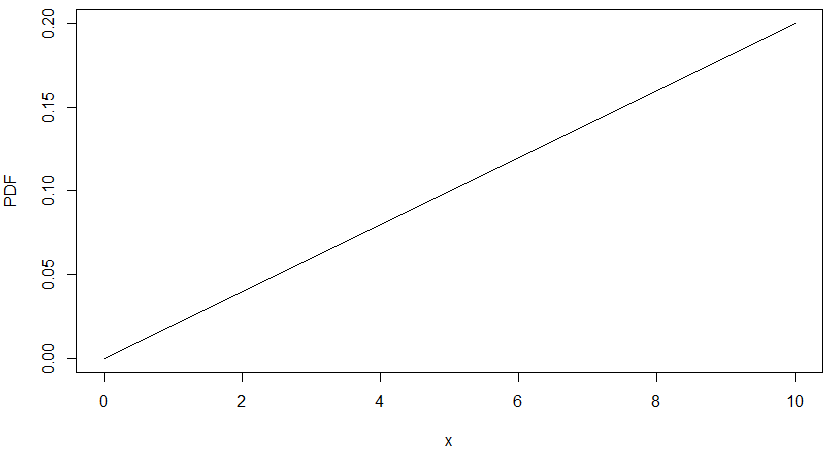
\includegraphics[scale=0.75]{images/PDF0.PNG}
    \caption{$f(x) = 0.02x$}
\end{figure}

\noindent
A PDF of $f(x) = 0.02x$ is valid because it is nonnegative within the interval of $[0, 10]$, and the area under this graph in that interval sums to 1.
To find $P(3 \leq X < 6)$ using simulations, we can use the following python code:

\begin{verbatim}
    # uniform distribution U ~ Unif(a, b)
    from random import uniform as unif

    # The PDF function f(x)
    def PDF(x):
        return 0.02 * x

    # lower bound
    a = 3

    # upper bound
    b = 6

    # maximum value of the PDF (or bigger)
    max = 0.2

    # number of trials
    n = 10000000

    # util
    num_false = 0
    num_true = 0
    x = 0
    y = 0

    # simulate using monte carlo
    for i in range(n):
        x = unif(a, b)
        y = unif(0, max)
        if y < PDF(x):
            num_true = num_true + 1
        else:
            num_false = num_false + 1

    # compute P(a <= X < b)
    P = (num_true / n) * (max * (b - a))
    print(P)
\end{verbatim}

\newpage
\noindent
This algorithm uses Monte Carlo simulations to estimate the probability.
We compute $n$ random points in interval [a, b] and count how many of them appear under the probability defined by the PDF.
To estimate the total probability, we use the following formula:

\[ \text{numberOfPointsUnderPDF} / n * \text{totalArea} \]

\noindent
Here the total area is computed as $maxHeight * (b - a)$.
Running this simulation for $n = 10000000$, it gives us an approximation of:

\[ P(3 \leq X < 6) = 0.2699601 \]

\subsection*{B}

\begin{itemize}
    \item The number of points $n$. Of course more points provides more accurate approximations.
    \item How accurate the uniform distribution is. If the distribution provided by the \textit{random} package from python isn't uniform then that infects the whole experiment.
\end{itemize}

\end{document}
